\documentclass[12pt,]{book}
\usepackage{lmodern}
\usepackage{setspace}
\setstretch{1.5}
\usepackage{amssymb,amsmath}
\usepackage{ifxetex,ifluatex}
\usepackage{fixltx2e} % provides \textsubscript
\ifnum 0\ifxetex 1\fi\ifluatex 1\fi=0 % if pdftex
  \usepackage[T1]{fontenc}
  \usepackage[utf8]{inputenc}
\else % if luatex or xelatex
  \ifxetex
    \usepackage{mathspec}
  \else
    \usepackage{fontspec}
  \fi
  \defaultfontfeatures{Ligatures=TeX,Scale=MatchLowercase}
\fi
% use upquote if available, for straight quotes in verbatim environments
\IfFileExists{upquote.sty}{\usepackage{upquote}}{}
% use microtype if available
\IfFileExists{microtype.sty}{%
\usepackage{microtype}
\UseMicrotypeSet[protrusion]{basicmath} % disable protrusion for tt fonts
}{}
\usepackage[margin=1in]{geometry}
\usepackage{hyperref}
\hypersetup{unicode=true,
            pdftitle={Data Science Workshop},
            pdfauthor={Alistair Bailey},
            pdfborder={0 0 0},
            breaklinks=true}
\urlstyle{same}  % don't use monospace font for urls
\usepackage{natbib}
\bibliographystyle{apalike}
\usepackage{color}
\usepackage{fancyvrb}
\newcommand{\VerbBar}{|}
\newcommand{\VERB}{\Verb[commandchars=\\\{\}]}
\DefineVerbatimEnvironment{Highlighting}{Verbatim}{commandchars=\\\{\}}
% Add ',fontsize=\small' for more characters per line
\usepackage{framed}
\definecolor{shadecolor}{RGB}{248,248,248}
\newenvironment{Shaded}{\begin{snugshade}}{\end{snugshade}}
\newcommand{\KeywordTok}[1]{\textcolor[rgb]{0.13,0.29,0.53}{\textbf{#1}}}
\newcommand{\DataTypeTok}[1]{\textcolor[rgb]{0.13,0.29,0.53}{#1}}
\newcommand{\DecValTok}[1]{\textcolor[rgb]{0.00,0.00,0.81}{#1}}
\newcommand{\BaseNTok}[1]{\textcolor[rgb]{0.00,0.00,0.81}{#1}}
\newcommand{\FloatTok}[1]{\textcolor[rgb]{0.00,0.00,0.81}{#1}}
\newcommand{\ConstantTok}[1]{\textcolor[rgb]{0.00,0.00,0.00}{#1}}
\newcommand{\CharTok}[1]{\textcolor[rgb]{0.31,0.60,0.02}{#1}}
\newcommand{\SpecialCharTok}[1]{\textcolor[rgb]{0.00,0.00,0.00}{#1}}
\newcommand{\StringTok}[1]{\textcolor[rgb]{0.31,0.60,0.02}{#1}}
\newcommand{\VerbatimStringTok}[1]{\textcolor[rgb]{0.31,0.60,0.02}{#1}}
\newcommand{\SpecialStringTok}[1]{\textcolor[rgb]{0.31,0.60,0.02}{#1}}
\newcommand{\ImportTok}[1]{#1}
\newcommand{\CommentTok}[1]{\textcolor[rgb]{0.56,0.35,0.01}{\textit{#1}}}
\newcommand{\DocumentationTok}[1]{\textcolor[rgb]{0.56,0.35,0.01}{\textbf{\textit{#1}}}}
\newcommand{\AnnotationTok}[1]{\textcolor[rgb]{0.56,0.35,0.01}{\textbf{\textit{#1}}}}
\newcommand{\CommentVarTok}[1]{\textcolor[rgb]{0.56,0.35,0.01}{\textbf{\textit{#1}}}}
\newcommand{\OtherTok}[1]{\textcolor[rgb]{0.56,0.35,0.01}{#1}}
\newcommand{\FunctionTok}[1]{\textcolor[rgb]{0.00,0.00,0.00}{#1}}
\newcommand{\VariableTok}[1]{\textcolor[rgb]{0.00,0.00,0.00}{#1}}
\newcommand{\ControlFlowTok}[1]{\textcolor[rgb]{0.13,0.29,0.53}{\textbf{#1}}}
\newcommand{\OperatorTok}[1]{\textcolor[rgb]{0.81,0.36,0.00}{\textbf{#1}}}
\newcommand{\BuiltInTok}[1]{#1}
\newcommand{\ExtensionTok}[1]{#1}
\newcommand{\PreprocessorTok}[1]{\textcolor[rgb]{0.56,0.35,0.01}{\textit{#1}}}
\newcommand{\AttributeTok}[1]{\textcolor[rgb]{0.77,0.63,0.00}{#1}}
\newcommand{\RegionMarkerTok}[1]{#1}
\newcommand{\InformationTok}[1]{\textcolor[rgb]{0.56,0.35,0.01}{\textbf{\textit{#1}}}}
\newcommand{\WarningTok}[1]{\textcolor[rgb]{0.56,0.35,0.01}{\textbf{\textit{#1}}}}
\newcommand{\AlertTok}[1]{\textcolor[rgb]{0.94,0.16,0.16}{#1}}
\newcommand{\ErrorTok}[1]{\textcolor[rgb]{0.64,0.00,0.00}{\textbf{#1}}}
\newcommand{\NormalTok}[1]{#1}
\usepackage{longtable,booktabs}
\usepackage{graphicx,grffile}
\makeatletter
\def\maxwidth{\ifdim\Gin@nat@width>\linewidth\linewidth\else\Gin@nat@width\fi}
\def\maxheight{\ifdim\Gin@nat@height>\textheight\textheight\else\Gin@nat@height\fi}
\makeatother
% Scale images if necessary, so that they will not overflow the page
% margins by default, and it is still possible to overwrite the defaults
% using explicit options in \includegraphics[width, height, ...]{}
\setkeys{Gin}{width=\maxwidth,height=\maxheight,keepaspectratio}
\IfFileExists{parskip.sty}{%
\usepackage{parskip}
}{% else
\setlength{\parindent}{0pt}
\setlength{\parskip}{6pt plus 2pt minus 1pt}
}
\setlength{\emergencystretch}{3em}  % prevent overfull lines
\providecommand{\tightlist}{%
  \setlength{\itemsep}{0pt}\setlength{\parskip}{0pt}}
\setcounter{secnumdepth}{5}
% Redefines (sub)paragraphs to behave more like sections
\ifx\paragraph\undefined\else
\let\oldparagraph\paragraph
\renewcommand{\paragraph}[1]{\oldparagraph{#1}\mbox{}}
\fi
\ifx\subparagraph\undefined\else
\let\oldsubparagraph\subparagraph
\renewcommand{\subparagraph}[1]{\oldsubparagraph{#1}\mbox{}}
\fi

%%% Use protect on footnotes to avoid problems with footnotes in titles
\let\rmarkdownfootnote\footnote%
\def\footnote{\protect\rmarkdownfootnote}

%%% Change title format to be more compact
\usepackage{titling}

% Create subtitle command for use in maketitle
\newcommand{\subtitle}[1]{
  \posttitle{
    \begin{center}\large#1\end{center}
    }
}

\setlength{\droptitle}{-2em}
  \title{Data Science Workshop}
  \pretitle{\vspace{\droptitle}\centering\huge}
  \posttitle{\par}
\subtitle{British Society for Proteomic Research Meeting 2018}
  \author{Alistair Bailey}
  \preauthor{\centering\large\emph}
  \postauthor{\par}
  \predate{\centering\large\emph}
  \postdate{\par}
  \date{May 29 2018}

\usepackage{booktabs}

% Preamble
\usepackage[none]{hyphenat}
\usepackage[default,osfigures,scale=0.95]{opensans} % Open sans font
\usepackage[T1]{fontenc} % Use 8-bit encoding that has 256 glyphs
\usepackage{lettrine} % The lettrine is the first enlarged letter at the beginning of the text
\raggedbottom 
\usepackage{makeidx} % These lines add bibliography to TOC
\makeindex
\usepackage[nottoc]{tocbibind}
\renewcommand{\bibname}{References} % Rename biblography as References

\usepackage{amsthm}
\newtheorem{theorem}{Theorem}[chapter]
\newtheorem{lemma}{Lemma}[chapter]
\theoremstyle{definition}
\newtheorem{definition}{Definition}[chapter]
\newtheorem{corollary}{Corollary}[chapter]
\newtheorem{proposition}{Proposition}[chapter]
\theoremstyle{definition}
\newtheorem{example}{Example}[chapter]
\theoremstyle{definition}
\newtheorem{exercise}{Exercise}[chapter]
\theoremstyle{remark}
\newtheorem*{remark}{Remark}
\newtheorem*{solution}{Solution}
\begin{document}
\maketitle

{
\setcounter{tocdepth}{1}
\tableofcontents
}
\chapter*{Overview}\label{overview}
\addcontentsline{toc}{chapter}{Overview}

These lessons cover:

\begin{enumerate}
\def\labelenumi{\arabic{enumi}.}
\tightlist
\item
  An introduction to R and RStudio
\item
  An introduction to the tidyverse
\item
  Importing and transforming proteomics data
\item
  Visualisation of proteomics analysis
\end{enumerate}

\section*{Requirements}\label{requirements}
\addcontentsline{toc}{section}{Requirements}

Up to date version of R and Rstudio

The following R packages:

\begin{Shaded}
\begin{Highlighting}[]
\KeywordTok{install.packages}\NormalTok{(}\KeywordTok{c}\NormalTok{(}\StringTok{"tidyverse"}\NormalTok{,}\StringTok{"janitor"}\NormalTok{))}
\end{Highlighting}
\end{Shaded}

\chapter{Introduction}\label{intro}

You can label chapter and section titles using \texttt{\{\#label\}}
after them, e.g., we can reference Chapter \ref{intro}. If you do not
manually label them, there will be automatic labels anyway, e.g.,
Chapter \ref{methods}.

Figures and tables with captions will be placed in \texttt{figure} and
\texttt{table} environments, respectively.

\begin{Shaded}
\begin{Highlighting}[]
\KeywordTok{par}\NormalTok{(}\DataTypeTok{mar =} \KeywordTok{c}\NormalTok{(}\DecValTok{4}\NormalTok{, }\DecValTok{4}\NormalTok{, .}\DecValTok{1}\NormalTok{, .}\DecValTok{1}\NormalTok{))}
\KeywordTok{plot}\NormalTok{(pressure, }\DataTypeTok{type =} \StringTok{'b'}\NormalTok{, }\DataTypeTok{pch =} \DecValTok{19}\NormalTok{)}
\end{Highlighting}
\end{Shaded}

\begin{figure}

{\centering 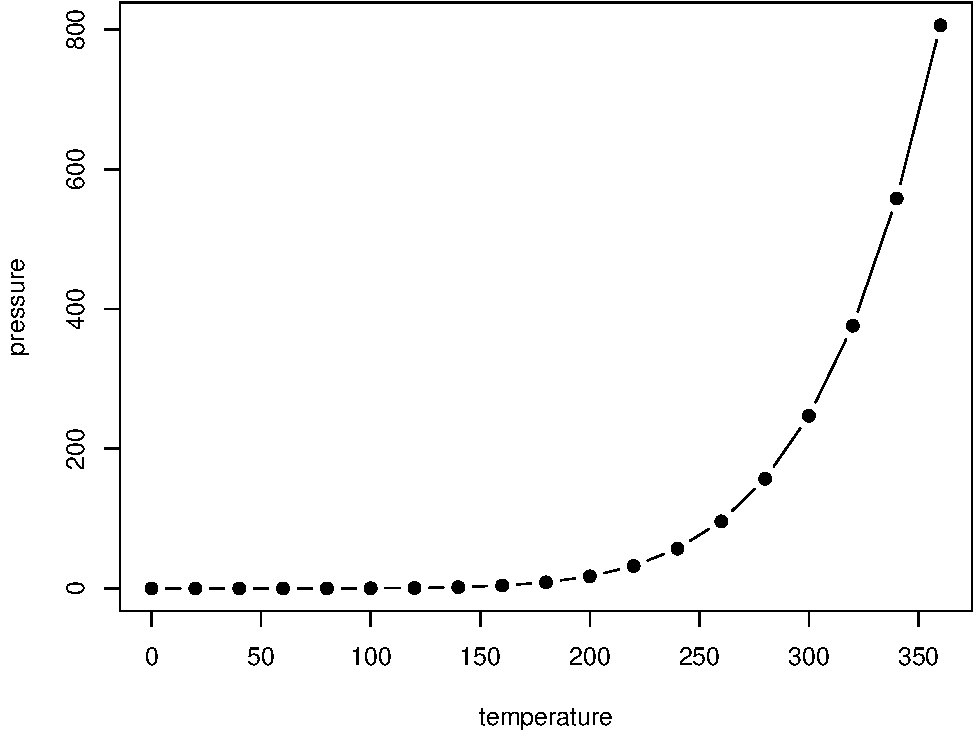
\includegraphics[width=0.8\linewidth]{bspr-workshop-2018_files/figure-latex/nice-fig-1} 

}

\caption{Here is a nice figure!}\label{fig:nice-fig}
\end{figure}

Reference a figure by its code chunk label with the \texttt{fig:}
prefix, e.g., see Figure \ref{fig:nice-fig}. Similarly, you can
reference tables generated from \texttt{knitr::kable()}, e.g., see Table
\ref{tab:nice-tab}.

\begin{Shaded}
\begin{Highlighting}[]
\NormalTok{knitr}\OperatorTok{::}\KeywordTok{kable}\NormalTok{(}
  \KeywordTok{head}\NormalTok{(iris, }\DecValTok{20}\NormalTok{), }\DataTypeTok{caption =} \StringTok{'Here is a nice table!'}\NormalTok{,}
  \DataTypeTok{booktabs =} \OtherTok{TRUE}
\NormalTok{)}
\end{Highlighting}
\end{Shaded}

\begin{table}

\caption{\label{tab:nice-tab}Here is a nice table!}
\centering
\begin{tabular}[t]{rrrrl}
\toprule
Sepal.Length & Sepal.Width & Petal.Length & Petal.Width & Species\\
\midrule
5.1 & 3.5 & 1.4 & 0.2 & setosa\\
4.9 & 3.0 & 1.4 & 0.2 & setosa\\
4.7 & 3.2 & 1.3 & 0.2 & setosa\\
4.6 & 3.1 & 1.5 & 0.2 & setosa\\
5.0 & 3.6 & 1.4 & 0.2 & setosa\\
\addlinespace
5.4 & 3.9 & 1.7 & 0.4 & setosa\\
4.6 & 3.4 & 1.4 & 0.3 & setosa\\
5.0 & 3.4 & 1.5 & 0.2 & setosa\\
4.4 & 2.9 & 1.4 & 0.2 & setosa\\
4.9 & 3.1 & 1.5 & 0.1 & setosa\\
\addlinespace
5.4 & 3.7 & 1.5 & 0.2 & setosa\\
4.8 & 3.4 & 1.6 & 0.2 & setosa\\
4.8 & 3.0 & 1.4 & 0.1 & setosa\\
4.3 & 3.0 & 1.1 & 0.1 & setosa\\
5.8 & 4.0 & 1.2 & 0.2 & setosa\\
\addlinespace
5.7 & 4.4 & 1.5 & 0.4 & setosa\\
5.4 & 3.9 & 1.3 & 0.4 & setosa\\
5.1 & 3.5 & 1.4 & 0.3 & setosa\\
5.7 & 3.8 & 1.7 & 0.3 & setosa\\
5.1 & 3.8 & 1.5 & 0.3 & setosa\\
\bottomrule
\end{tabular}
\end{table}

You can write citations, too. For example, we are using the
\textbf{bookdown} package \citep{R-bookdown} in this sample book, which
was built on top of R Markdown and \textbf{knitr} \citep{xie2015}.

\chapter{The tidyverse}\label{the-tidyverse}

An introduction to the tidyverse.

\chapter{Importing and transforming proteomics
data}\label{importing-and-transforming-proteomics-data}

\section{Importing flat files}\label{importing-flat-files}

\section{Calculating fold change and
enrichment}\label{calculating-fold-change-and-enrichment}

\subsection{Fold change and log-fold
change}\label{fold-change-and-log-fold-change}

Fold changes are ratios, the ratio of say protein expression before and
after treatment, where a value larger than 1 for a protein implies that
protein expression was greater after the treatment.

In life sciences, fold change is often reported as log-fold change. Why
is that? There are at least two reasons which can be shown by plotting.

One is that ratios are not symmetrical around 1, so it's difficult to
observe both changes in the forwards and backwards direcion
i.e.~proteins where expression went up and proteins where expression
went down due to treatment. When we transform ratios on a log scale, the
scale becomes symmetric around 0 and thus we can now observe the
distribution of ratios in terms of positive, negative or no change.

\begin{Shaded}
\begin{Highlighting}[]
\KeywordTok{set.seed}\NormalTok{(}\DecValTok{10}\NormalTok{)}
\NormalTok{x <-}\StringTok{ }\DecValTok{2}\OperatorTok{^}\NormalTok{(}\KeywordTok{rnorm}\NormalTok{(}\DecValTok{100}\NormalTok{))}
\NormalTok{y <-}\StringTok{ }\DecValTok{2}\OperatorTok{^}\NormalTok{(}\KeywordTok{rnorm}\NormalTok{(}\DecValTok{100}\NormalTok{))}
\NormalTok{ratios <-}\StringTok{ }\KeywordTok{tibble}\NormalTok{(}\DataTypeTok{value =}\NormalTok{ x}\OperatorTok{/}\NormalTok{y, }\DataTypeTok{label =} \StringTok{"ratios"}\NormalTok{)}
\NormalTok{logratios <-}\StringTok{ }\KeywordTok{tibble}\NormalTok{(}\DataTypeTok{value =} \KeywordTok{log2}\NormalTok{(ratios}\OperatorTok{$}\NormalTok{value), }\DataTypeTok{label =} \StringTok{"logratios"}\NormalTok{)}

\KeywordTok{bind_rows}\NormalTok{(ratios,logratios) }\OperatorTok\StringTok{ }
\StringTok{  }\KeywordTok{ggplot}\NormalTok{(}\KeywordTok{aes}\NormalTok{(value)) }\OperatorTok{+}
\StringTok{  }\KeywordTok{geom_histogram}\NormalTok{(}\DataTypeTok{binwidth =} \DecValTok{2}\NormalTok{, }\DataTypeTok{colour =} \StringTok{"grey50"}\NormalTok{, }\DataTypeTok{fill =} \StringTok{"white"}\NormalTok{) }\OperatorTok{+}
\StringTok{  }\NormalTok{ggplot2}\OperatorTok{::}\KeywordTok{facet_wrap}\NormalTok{(}\OperatorTok{~}\StringTok{ }\NormalTok{label) }\OperatorTok{+}
\StringTok{  }\KeywordTok{theme_minimal}\NormalTok{()}
\end{Highlighting}
\end{Shaded}

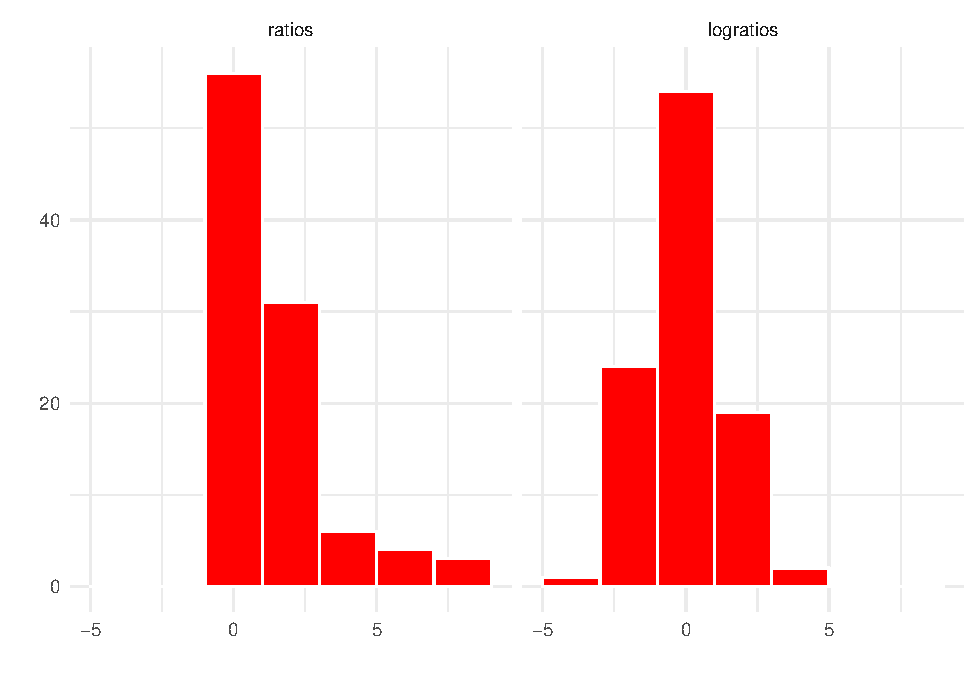
\includegraphics{bspr-workshop-2018_files/figure-latex/fold-change-1-1.pdf}

A second reason is that transforming values onto a log scale changes
where the numbers actually occur when plotted on that scale. If we
consider the log scale to represent magnitudes, then we can more easily
see changes of small and large magnitudes when we plot the data.

For example, a fold change of 32 times can be either a ratio 1/32 or
32/1.

1/32 is much closer to 1 than 32/1, but transformed to a log scale we
see that in terms of magnitude of difference it is the same as 32/1.

\begin{Shaded}
\begin{Highlighting}[]
\NormalTok{x2 <-}\StringTok{ }\DecValTok{2}\OperatorTok{^}\KeywordTok{seq}\NormalTok{(}\DecValTok{1}\NormalTok{,}\DecValTok{5}\NormalTok{)}
\NormalTok{y_vals <-}\StringTok{ }\KeywordTok{c}\NormalTok{(}\KeywordTok{rev}\NormalTok{(}\DecValTok{1}\OperatorTok{/}\NormalTok{x2),}\DecValTok{1}\NormalTok{,x2)}
\NormalTok{names <-}\StringTok{ }\KeywordTok{c}\NormalTok{(}\KeywordTok{paste0}\NormalTok{(}\StringTok{"1/"}\NormalTok{,}\KeywordTok{rev}\NormalTok{(x2)),}\DecValTok{1}\NormalTok{,x2)}
\NormalTok{x_vals <-}\StringTok{ }\KeywordTok{seq}\NormalTok{(}\DataTypeTok{along=}\NormalTok{y_vals)}

\NormalTok{dat <-}\StringTok{ }\KeywordTok{tibble}\NormalTok{(x_vals,y_vals,names)}

\NormalTok{p1 <-}\StringTok{ }\KeywordTok{ggplot}\NormalTok{(dat,}\KeywordTok{aes}\NormalTok{(x_vals,y_vals, }\DataTypeTok{label =}\NormalTok{ names)) }\OperatorTok{+}
\StringTok{  }\KeywordTok{geom_text}\NormalTok{() }\OperatorTok{+}
\StringTok{  }\KeywordTok{geom_hline}\NormalTok{(}\DataTypeTok{yintercept =} \DecValTok{1}\NormalTok{) }\OperatorTok{+}
\StringTok{  }\KeywordTok{theme_minimal}\NormalTok{() }\OperatorTok{+}
\StringTok{  }\KeywordTok{labs}\NormalTok{(}\DataTypeTok{x =} \OtherTok{NULL}\NormalTok{, }\DataTypeTok{y =} \OtherTok{NULL}\NormalTok{) }\OperatorTok{+}
\StringTok{  }\KeywordTok{scale_x_continuous}\NormalTok{(}\DataTypeTok{breaks =} \OtherTok{NULL}\NormalTok{)}


\NormalTok{p2 <-}\StringTok{ }\KeywordTok{ggplot}\NormalTok{(dat,}\KeywordTok{aes}\NormalTok{(x_vals,y_vals, }\DataTypeTok{label =}\NormalTok{ names)) }\OperatorTok{+}
\StringTok{  }\KeywordTok{geom_text}\NormalTok{() }\OperatorTok{+}
\StringTok{  }\KeywordTok{geom_hline}\NormalTok{(}\DataTypeTok{yintercept =} \DecValTok{1}\NormalTok{) }\OperatorTok{+}
\StringTok{  }\KeywordTok{scale_y_continuous}\NormalTok{(}\DataTypeTok{trans =} \StringTok{"log2"}\NormalTok{) }\OperatorTok{+}
\StringTok{  }\KeywordTok{theme_minimal}\NormalTok{() }\OperatorTok{+}
\StringTok{  }\KeywordTok{labs}\NormalTok{(}\DataTypeTok{x =} \OtherTok{NULL}\NormalTok{, }\DataTypeTok{y =} \OtherTok{NULL}\NormalTok{) }\OperatorTok{+}
\StringTok{  }\KeywordTok{scale_x_continuous}\NormalTok{(}\DataTypeTok{breaks =} \OtherTok{NULL}\NormalTok{)}

\KeywordTok{plot_grid}\NormalTok{(p1,p2)}
\end{Highlighting}
\end{Shaded}

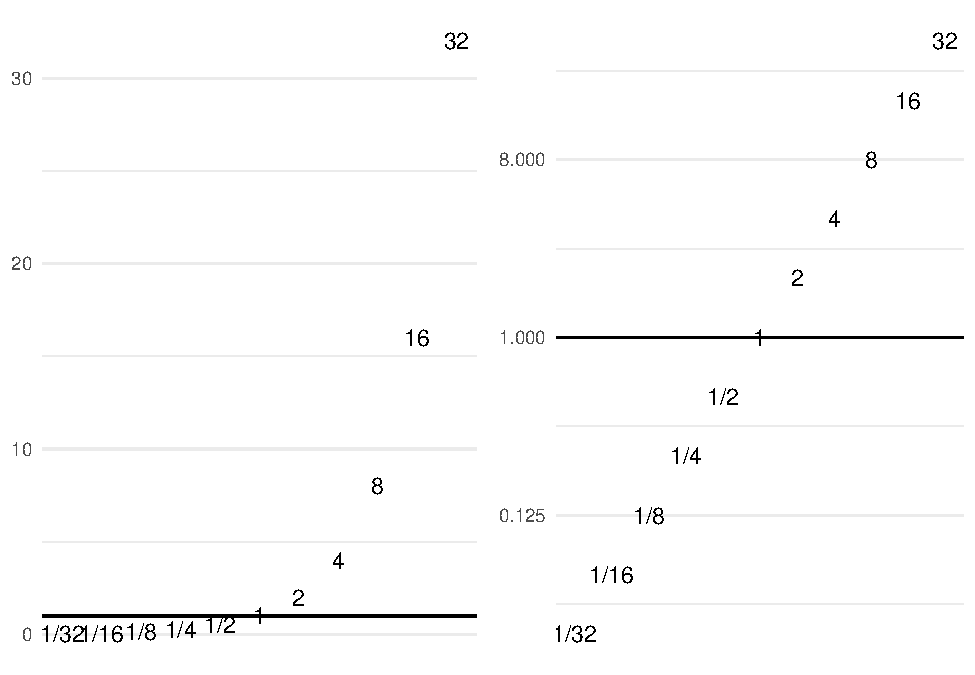
\includegraphics{bspr-workshop-2018_files/figure-latex/fold-change-2-1.pdf}

\chapter{Fold change and t-test}\label{fold-change-and-t-test}

\begin{enumerate}
\def\labelenumi{\arabic{enumi}.}
\tightlist
\item
  Load the data, we need multiple replicates for each condition. To be
  tidy each protein is a set of observations (rows) of the variables,
  which are the values recorded for each replicate (columns).
\end{enumerate}

\begin{verbatim}
## Parsed with column specification:
## cols(
##   protein.key_protein.Accession = col_character(),
##   protein.Description = col_character(),
##   `protein.ngramOnColumn -> EmillyBowler_KOGSK_Rep1_001_Merged_Spectrum_IA_final_protein` = col_double(),
##   `protein.ngramOnColumn -> EmillyBowler_KOGSK_Rep2_Merged_IA_final_protein` = col_double(),
##   `protein.ngramOnColumn -> EmillyBowler_KOGSK_Rep3_001_Merged_Spectrum_IA_final_protein` = col_double(),
##   `protein.ngramOnColumn -> EmillyBowler_WT_Rep1_001_Merged_Spectrum_IA_final_protein` = col_double(),
##   `protein.ngramOnColumn -> EmillyBowler_WT_Rep2_001_Merged_Spectrum_IA_final_protein` = col_double(),
##   `protein.ngramOnColumn -> EmillyBowler_WT_Rep3_001_Merged_Spectrum_IA_final_protein` = col_double(),
##   Present_NumFiles = col_integer()
## )
\end{verbatim}

\begin{verbatim}
## Observations: 6,150
## Variables: 9
## $ protein_key_protein_accession                                                         <chr> ...
## $ protein_description                                                                   <chr> ...
## $ protein_ngram_on_column_emilly_bowler_kogsk_rep1_001_merged_spectrum_ia_final_protein <dbl> ...
## $ protein_ngram_on_column_emilly_bowler_kogsk_rep2_merged_ia_final_protein              <dbl> ...
## $ protein_ngram_on_column_emilly_bowler_kogsk_rep3_001_merged_spectrum_ia_final_protein <dbl> ...
## $ protein_ngram_on_column_emilly_bowler_wt_rep1_001_merged_spectrum_ia_final_protein    <dbl> ...
## $ protein_ngram_on_column_emilly_bowler_wt_rep2_001_merged_spectrum_ia_final_protein    <dbl> ...
## $ protein_ngram_on_column_emilly_bowler_wt_rep3_001_merged_spectrum_ia_final_protein    <dbl> ...
## $ present_num_files                                                                     <int> ...
\end{verbatim}

\begin{enumerate}
\def\labelenumi{\arabic{enumi}.}
\setcounter{enumi}{1}
\tightlist
\item
  Tidy up and deal with missing values, either impute or exclude missing
  values and normalise.
\end{enumerate}

Let's consider our proteomics data as a distribution of values, one
value for each protein in our experiment that together form a
distribution. If we have replicate experiments we'll therefore have
multiple distributions.

A quantile represents a region of distribution, for example the 0.95
quantile is the value such that 95\% of the data lies below it. To
normalise two or more distributions with each other without recourse to
a reference distribution we:

\begin{enumerate}
\def\labelenumi{(\roman{enumi})}
\tightlist
\item
  Rank (quantile) the value in each experiment (column) from lowest to
  highest.
\item
  Sort each experiment (column) from lowest to highest value.
\item
  Calculate the mean across the experiments (rows) on the sorted values.
\item
  Substitute the mean values according to rank for each experiment to
  restore the original order.
\end{enumerate}

\href{https://davetang.org/muse/2014/07/07/quantile-normalisation-in-r/}{Dave
Tang's Blog : Quantile Normalisation in R}

.\citet{ewanbirney} Neither corresponds to the \citet{Bioconductor}
implementation of quantile norm (est 2001 and explained below)
pic.twitter.com/lCyy6YyNB8

--- Rafael Irizarry (\citet{rafalab}) December 18, 2014

\begin{Shaded}
\begin{Highlighting}[]
\CommentTok{# Tidy data up}
\NormalTok{dat_tidy <-}\StringTok{ }\NormalTok{dat_em }\OperatorTok
\StringTok{  }\CommentTok{# Remove missing values}
\StringTok{  }\KeywordTok{drop_na}\NormalTok{() }\OperatorTok\StringTok{ }
\StringTok{  }\CommentTok{# Select and rename columns}
\StringTok{  }\KeywordTok{select}\NormalTok{(}\DataTypeTok{protein_accession =}\NormalTok{ protein_key_protein_accession,}
\NormalTok{         protein_description,}
         \DataTypeTok{wt1 =}\NormalTok{ protein_ngram_on_column_emilly_bowler_wt_rep1_001_merged_spectrum_ia_final_protein,}
         \DataTypeTok{wt2 =}\NormalTok{ protein_ngram_on_column_emilly_bowler_wt_rep2_001_merged_spectrum_ia_final_protein,}
         \DataTypeTok{wt3 =}\NormalTok{ protein_ngram_on_column_emilly_bowler_wt_rep3_001_merged_spectrum_ia_final_protein,}
         \DataTypeTok{kog1 =}\NormalTok{ protein_ngram_on_column_emilly_bowler_kogsk_rep1_001_merged_spectrum_ia_final_protein,}
         \DataTypeTok{kog2 =}\NormalTok{ protein_ngram_on_column_emilly_bowler_kogsk_rep2_merged_ia_final_protein,}
         \DataTypeTok{kog3 =}\NormalTok{ protein_ngram_on_column_emilly_bowler_kogsk_rep3_001_merged_spectrum_ia_final_protein)}

\CommentTok{# Plot data}
\NormalTok{dat_tidy }\OperatorTok\StringTok{ }
\StringTok{  }\KeywordTok{ggplot}\NormalTok{(}\KeywordTok{aes}\NormalTok{(}\KeywordTok{log2}\NormalTok{(wt1))) }\OperatorTok{+}\StringTok{ }
\StringTok{  }\KeywordTok{geom_density}\NormalTok{() }\OperatorTok{+}
\StringTok{  }\KeywordTok{geom_density}\NormalTok{(}\KeywordTok{aes}\NormalTok{(}\KeywordTok{log2}\NormalTok{(wt2), }\DataTypeTok{colour =} \StringTok{"blue"}\NormalTok{)) }\OperatorTok{+}
\StringTok{  }\KeywordTok{geom_density}\NormalTok{(}\KeywordTok{aes}\NormalTok{(}\KeywordTok{log2}\NormalTok{(wt3), }\DataTypeTok{colour =} \StringTok{"red"}\NormalTok{))}
\end{Highlighting}
\end{Shaded}

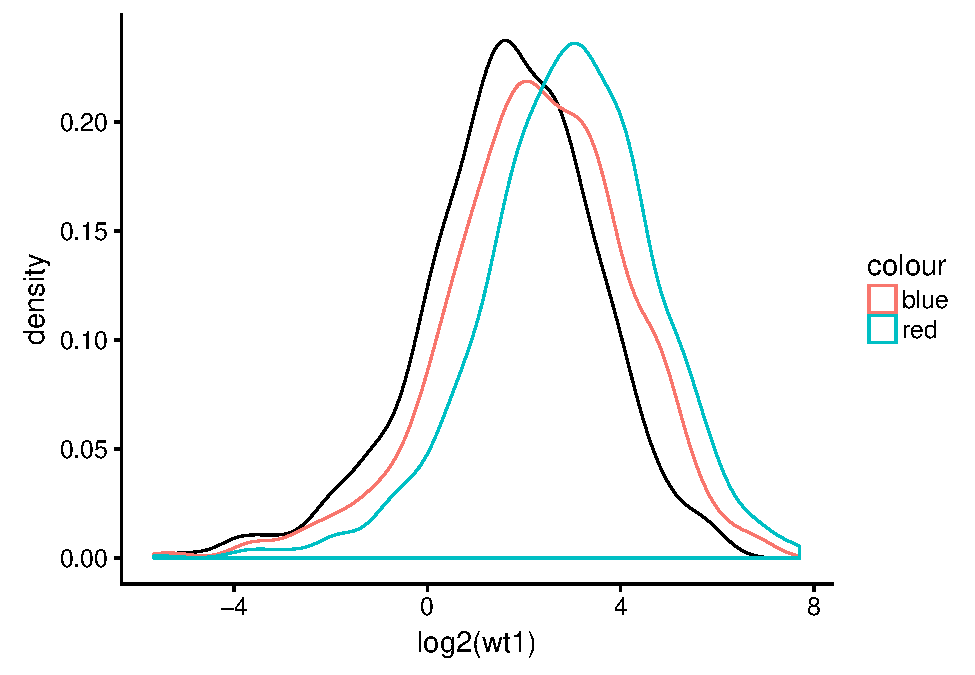
\includegraphics{bspr-workshop-2018_files/figure-latex/tidy-data-1.pdf}

\begin{Shaded}
\begin{Highlighting}[]
\CommentTok{# Normalise to maximum column value}
\NormalTok{dat_norm_max <-}\StringTok{ }\NormalTok{dat_tidy }\OperatorTok\StringTok{ }
\StringTok{  }\KeywordTok{mutate}\NormalTok{(}\DataTypeTok{wt1 =}\NormalTok{ wt1}\OperatorTok{/}\KeywordTok{max}\NormalTok{(wt1),}
         \DataTypeTok{wt2 =}\NormalTok{ wt2}\OperatorTok{/}\KeywordTok{max}\NormalTok{(wt3),}
         \DataTypeTok{wt3 =}\NormalTok{ wt3}\OperatorTok{/}\KeywordTok{max}\NormalTok{(wt3),}
         \DataTypeTok{kog1 =}\NormalTok{ kog1 }\OperatorTok{/}\StringTok{ }\KeywordTok{max}\NormalTok{(kog1),}
         \DataTypeTok{kog2 =}\NormalTok{ kog2 }\OperatorTok{/}\StringTok{ }\KeywordTok{max}\NormalTok{(kog2),}
         \DataTypeTok{kog3 =}\NormalTok{ kog3 }\OperatorTok{/}\StringTok{ }\KeywordTok{max}\NormalTok{(kog3)}
\NormalTok{         )}

\CommentTok{# Normalise to median column value}
\NormalTok{dat_norm_med <-}\StringTok{ }\NormalTok{dat_tidy }\OperatorTok\StringTok{ }
\StringTok{  }\KeywordTok{mutate}\NormalTok{(}\DataTypeTok{wt1 =}\NormalTok{ wt1}\OperatorTok{/}\KeywordTok{median}\NormalTok{(wt1),}
         \DataTypeTok{wt2 =}\NormalTok{ wt2}\OperatorTok{/}\KeywordTok{median}\NormalTok{(wt3),}
         \DataTypeTok{wt3 =}\NormalTok{ wt3}\OperatorTok{/}\KeywordTok{median}\NormalTok{(wt3),}
         \DataTypeTok{kog1 =}\NormalTok{ kog1 }\OperatorTok{/}\StringTok{ }\KeywordTok{median}\NormalTok{(kog1),}
         \DataTypeTok{kog2 =}\NormalTok{ kog2 }\OperatorTok{/}\StringTok{ }\KeywordTok{median}\NormalTok{(kog2),}
         \DataTypeTok{kog3 =}\NormalTok{ kog3 }\OperatorTok{/}\StringTok{ }\KeywordTok{median}\NormalTok{(kog3)}
\NormalTok{         )}

\NormalTok{dat_rank <-}\StringTok{ }\NormalTok{dat_tidy }\OperatorTok\StringTok{ }\KeywordTok{select}\NormalTok{(}\OperatorTok{-}\KeywordTok{c}\NormalTok{(}\DecValTok{1}\OperatorTok{:}\DecValTok{2}\NormalTok{,}\DecValTok{6}\OperatorTok{:}\DecValTok{8}\NormalTok{)) }\OperatorTok\StringTok{ }
\StringTok{  }\KeywordTok{apply}\NormalTok{(., }\DecValTok{2}\NormalTok{, rank, }\DataTypeTok{ties.method=}\StringTok{"min"}\NormalTok{) }\OperatorTok\StringTok{ }\KeywordTok{as.data.frame}\NormalTok{()}

\NormalTok{dat_sort <-}\StringTok{ }\NormalTok{dat_tidy }\OperatorTok\StringTok{ }\KeywordTok{select}\NormalTok{(}\OperatorTok{-}\KeywordTok{c}\NormalTok{(}\DecValTok{1}\OperatorTok{:}\DecValTok{2}\NormalTok{,}\DecValTok{6}\OperatorTok{:}\DecValTok{8}\NormalTok{)) }\OperatorTok\StringTok{ }
\StringTok{  }\KeywordTok{apply}\NormalTok{(., }\DecValTok{2}\NormalTok{, sort) }\OperatorTok\StringTok{ }\KeywordTok{as.data.frame}\NormalTok{()}

\NormalTok{dat_mean <-}\StringTok{ }\NormalTok{dat_sort }\OperatorTok\StringTok{ }\KeywordTok{apply}\NormalTok{(., }\DecValTok{1}\NormalTok{, mean)}

\NormalTok{index_mean <-}\StringTok{ }\ControlFlowTok{function}\NormalTok{(my_idx, my_mean)\{}
  \KeywordTok{return}\NormalTok{(my_mean[my_idx])}
\NormalTok{\}}

\NormalTok{dat_norm <-}\StringTok{ }\NormalTok{dat_rank }\OperatorTok\StringTok{ }
\StringTok{  }\KeywordTok{apply}\NormalTok{(.,}\DecValTok{2}\NormalTok{,index_mean, }\DataTypeTok{my_mean =}\NormalTok{ dat_mean) }\OperatorTok\StringTok{ }
\StringTok{  }\KeywordTok{as.data.frame}\NormalTok{()}

\CommentTok{# dat_wt %>% }
\CommentTok{#   ggplot(aes(log2(wt1))) + }
\CommentTok{#   geom_density() +}
\CommentTok{#   geom_density(aes(log2(wt2), colour = "blue")) +}
\CommentTok{#   geom_density(aes(log2(wt3), colour = "red"))}

\CommentTok{# Quantile normalisation : the aim is to give different distributions the}
\CommentTok{# same statistical properties}
\NormalTok{quantile_normalisation <-}\StringTok{ }\ControlFlowTok{function}\NormalTok{(df)\{}
  \CommentTok{#}
\NormalTok{  df_rank <-}\StringTok{ }\KeywordTok{apply}\NormalTok{(df,}\DecValTok{2}\NormalTok{,rank,}\DataTypeTok{ties.method=}\StringTok{"average"}\NormalTok{)}
\NormalTok{  df_sorted <-}\StringTok{ }\KeywordTok{data.frame}\NormalTok{(}\KeywordTok{apply}\NormalTok{(df, }\DecValTok{2}\NormalTok{, sort))}
\NormalTok{  df_mean <-}\StringTok{ }\KeywordTok{apply}\NormalTok{(df_sorted, }\DecValTok{1}\NormalTok{, mean)}
   
\NormalTok{  index_to_mean <-}\StringTok{ }\ControlFlowTok{function}\NormalTok{(my_index, my_mean)\{}
    \KeywordTok{return}\NormalTok{(my_mean[my_index])}
\NormalTok{  \}}
   
\NormalTok{  df_final <-}\StringTok{ }\KeywordTok{apply}\NormalTok{(df_rank, }\DecValTok{2}\NormalTok{, index_to_mean, }\DataTypeTok{my_mean=}\NormalTok{df_mean) }\OperatorTok\StringTok{ }\KeywordTok{as.data.frame}\NormalTok{()}
  \CommentTok{#rownames(df_final) <- rownames(df)}
  \KeywordTok{return}\NormalTok{(df_final)}
\NormalTok{\}}

\NormalTok{dt_wt <-}\StringTok{ }\NormalTok{dat_tidy }\OperatorTok\StringTok{ }\KeywordTok{select}\NormalTok{(}\OperatorTok{-}\KeywordTok{c}\NormalTok{(}\DecValTok{1}\OperatorTok{:}\DecValTok{2}\NormalTok{,}\DecValTok{6}\OperatorTok{:}\DecValTok{8}\NormalTok{))}
\NormalTok{dt_kog <-}\StringTok{ }\NormalTok{dat_tidy }\OperatorTok\StringTok{ }\KeywordTok{select}\NormalTok{(}\OperatorTok{-}\KeywordTok{c}\NormalTok{(}\DecValTok{1}\OperatorTok{:}\DecValTok{5}\NormalTok{))}

\NormalTok{dt_wt_norm <-}\StringTok{ }\KeywordTok{quantile_normalisation}\NormalTok{(dt_wt)}
\NormalTok{dt_kog_norm <-}\StringTok{ }\KeywordTok{quantile_normalisation}\NormalTok{(dt_kog)}

\NormalTok{dat_norm <-}\StringTok{ }\KeywordTok{bind_cols}\NormalTok{(dat_tidy[,}\DecValTok{1}\OperatorTok{:}\DecValTok{2}\NormalTok{],dt_wt_norm,dt_kog_norm)}
\CommentTok{# Have a look at the median normalised data}
\KeywordTok{glimpse}\NormalTok{(dat_norm_med)}
\end{Highlighting}
\end{Shaded}

\begin{verbatim}
## Observations: 1,095
## Variables: 8
## $ protein_accession   <chr> "4562_DHE3_HUMAN", "14948_RS2_HUMAN", "143...
## $ protein_description <chr> "Glutamate dehydrogenase 1_ mitochondrial ...
## $ wt1                 <dbl> 1.46455644, 3.78274902, 0.10257018, 1.5593...
## $ wt2                 <dbl> 1.29015126, 3.06162560, 0.06677263, 1.2956...
## $ wt3                 <dbl> 1.3898245, 4.6907618, 0.1136384, 0.7625680...
## $ kog1                <dbl> 2.1246421, 2.2498354, 0.2868330, 0.9172013...
## $ kog2                <dbl> 0.06248655, 3.78198563, 0.08551018, 0.5341...
## $ kog3                <dbl> 1.55811005, 2.16717459, 0.32849794, 0.8012...
\end{verbatim}

\begin{Shaded}
\begin{Highlighting}[]
\CommentTok{# Save the median normalised data}
\KeywordTok{write_excel_csv}\NormalTok{(dat_norm,}\StringTok{"data/example_median_nomralised_proteomics_data.csv"}\NormalTok{)}
\end{Highlighting}
\end{Shaded}

\begin{Shaded}
\begin{Highlighting}[]
\CommentTok{# Impute NA with lowest value, need to change this!}
\NormalTok{control <-}\StringTok{ }\NormalTok{dat_select }\OperatorTok\StringTok{ }\KeywordTok{filter}\NormalTok{(}\OperatorTok{!}\KeywordTok{is.na}\NormalTok{(control_}\DecValTok{1}\NormalTok{) }\OperatorTok{|}\StringTok{ }
\StringTok{                                   }\OperatorTok{!}\KeywordTok{is.na}\NormalTok{(control_}\DecValTok{2}\NormalTok{) }\OperatorTok{|}\StringTok{ }
\StringTok{                                   }\OperatorTok{!}\KeywordTok{is.na}\NormalTok{(control_}\DecValTok{3}\NormalTok{)) }\OperatorTok\StringTok{ }\KeywordTok{select}\NormalTok{(}\DecValTok{3}\NormalTok{,}\DecValTok{4}\NormalTok{,}\DecValTok{5}\NormalTok{) }

\NormalTok{treatment <-}\StringTok{ }\NormalTok{dat_select }\OperatorTok\StringTok{ }\KeywordTok{filter}\NormalTok{(}\OperatorTok{!}\KeywordTok{is.na}\NormalTok{(ras_}\DecValTok{1}\NormalTok{) }\OperatorTok{|}\StringTok{ }
\StringTok{                                   }\OperatorTok{!}\KeywordTok{is.na}\NormalTok{(ras_}\DecValTok{2}\NormalTok{) }\OperatorTok{|}\StringTok{ }
\StringTok{                                   }\OperatorTok{!}\KeywordTok{is.na}\NormalTok{(ras_}\DecValTok{3}\NormalTok{)) }\OperatorTok\StringTok{ }\KeywordTok{select}\NormalTok{(}\DecValTok{6}\NormalTok{,}\DecValTok{7}\NormalTok{,}\DecValTok{8}\NormalTok{) }

\CommentTok{# Impute minimum}
\NormalTok{row_min <-}\StringTok{ }\ControlFlowTok{function}\NormalTok{(x) }\KeywordTok{apply}\NormalTok{(x,}\DecValTok{1}\NormalTok{,min,}\DataTypeTok{na.rm =} \OtherTok{TRUE}\NormalTok{)}
\NormalTok{impute_min <-}\StringTok{ }\ControlFlowTok{function}\NormalTok{(x) }\KeywordTok{replace}\NormalTok{(x, }\KeywordTok{is.na}\NormalTok{(x), }\KeywordTok{row_min}\NormalTok{(x))}

\CommentTok{#control_na <- control %>% filter(!complete.cases(.))}
\KeywordTok{impute_min}\NormalTok{(control)}

 
\NormalTok{control }\OperatorTok\StringTok{ }\KeywordTok{replace_na}\NormalTok{(}\KeywordTok{apply}\NormalTok{(.,}\DecValTok{1}\NormalTok{,min))}
\end{Highlighting}
\end{Shaded}

\begin{enumerate}
\def\labelenumi{\arabic{enumi}.}
\setcounter{enumi}{2}
\tightlist
\item
  Use \texttt{t.test} to perform Welch Two Sample t-test on
  untransformed data. This outputs the p-values we need for each
  protein.
\end{enumerate}

\begin{Shaded}
\begin{Highlighting}[]
\CommentTok{# T-test function for multiple experiments}
\NormalTok{expriments_ttest <-}\StringTok{ }\ControlFlowTok{function}\NormalTok{(dt,grp1,grp2)\{}
  \CommentTok{# Subset control group and convert to numeric}
\NormalTok{  x <-}\StringTok{ }\NormalTok{dt[grp1] }\OperatorTok\StringTok{ }\NormalTok{unlist }\OperatorTok\StringTok{ }\KeywordTok{as.numeric}\NormalTok{()}
  \CommentTok{# Subset treatment group and convert to numeric}
\NormalTok{  y <-}\StringTok{ }\NormalTok{dt[grp2] }\OperatorTok\StringTok{ }\NormalTok{unlist }\OperatorTok\StringTok{ }\KeywordTok{as.numeric}\NormalTok{()}
  \CommentTok{# Perform t-test}
\NormalTok{  result <-}\StringTok{ }\KeywordTok{t.test}\NormalTok{(x, y)}
  \CommentTok{# Return p-values}
  \KeywordTok{return}\NormalTok{(result}\OperatorTok{$}\NormalTok{p.value)}
\NormalTok{\}  }

\CommentTok{# Apply t-test function to data}
\CommentTok{# array = dat, 1 = rows, FUN = expriments_ttest, and arguements}
\CommentTok{# For median normalised data}
\NormalTok{p_vals <-}\StringTok{ }\KeywordTok{apply}\NormalTok{(dat_norm,}\DecValTok{1}\NormalTok{,expriments_ttest, }\DataTypeTok{grp1 =} \KeywordTok{c}\NormalTok{(}\DecValTok{3}\OperatorTok{:}\DecValTok{5}\NormalTok{), }\DataTypeTok{grp2 =} \KeywordTok{c}\NormalTok{(}\DecValTok{6}\OperatorTok{:}\DecValTok{8}\NormalTok{))}
\CommentTok{# For maximum normalised data}
\NormalTok{p_vals_max <-}\StringTok{ }\KeywordTok{apply}\NormalTok{(dat_norm_max,}\DecValTok{1}\NormalTok{,expriments_ttest, }\DataTypeTok{grp1 =} \KeywordTok{c}\NormalTok{(}\DecValTok{3}\OperatorTok{:}\DecValTok{5}\NormalTok{), }\DataTypeTok{grp2 =} \KeywordTok{c}\NormalTok{(}\DecValTok{6}\OperatorTok{:}\DecValTok{8}\NormalTok{))}

\CommentTok{# Plot histograms}
\KeywordTok{hist}\NormalTok{(p_vals)}
\end{Highlighting}
\end{Shaded}

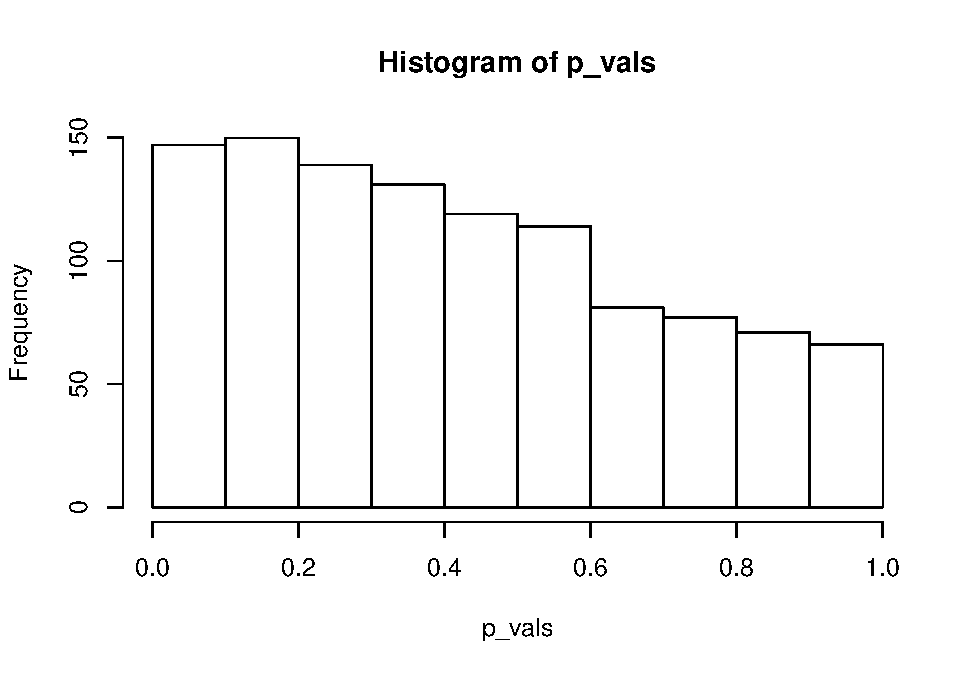
\includegraphics{bspr-workshop-2018_files/figure-latex/t-test-1.pdf}

\begin{Shaded}
\begin{Highlighting}[]
\KeywordTok{hist}\NormalTok{(p_vals_max)}
\end{Highlighting}
\end{Shaded}

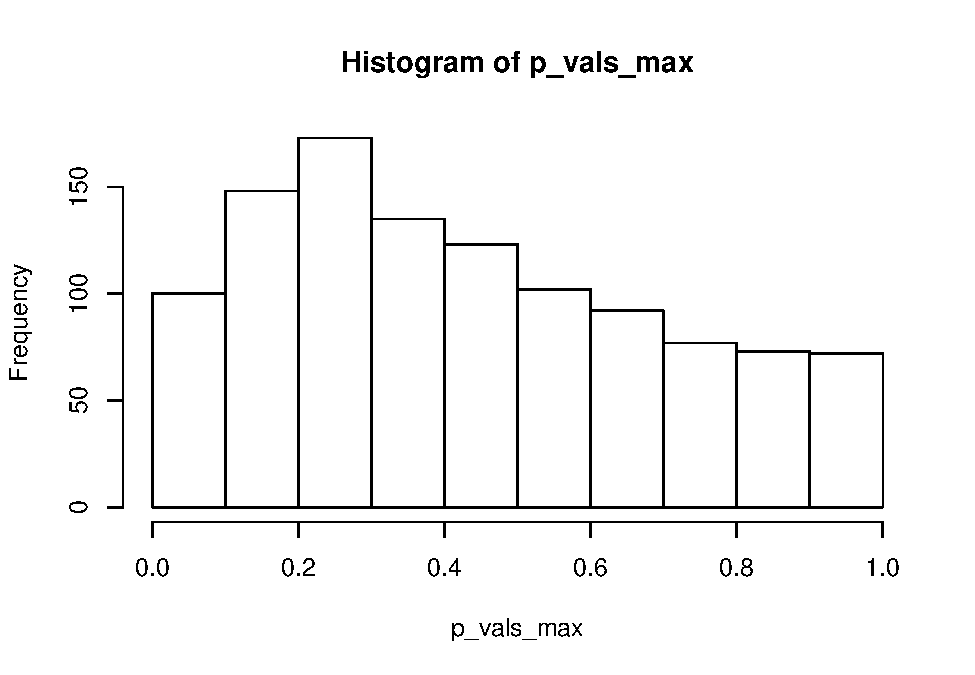
\includegraphics{bspr-workshop-2018_files/figure-latex/t-test-2.pdf}

\begin{enumerate}
\def\labelenumi{\arabic{enumi}.}
\setcounter{enumi}{3}
\tightlist
\item
  Perform log transformation of the observations for each protein.
\end{enumerate}

\begin{Shaded}
\begin{Highlighting}[]
\CommentTok{# Select columns and log data}
\NormalTok{dat_log <-}\StringTok{ }\NormalTok{dat_norm }\OperatorTok\StringTok{ }
\StringTok{  }\KeywordTok{select}\NormalTok{(}\OperatorTok{-}\KeywordTok{c}\NormalTok{(protein_accession,protein_description)) }\OperatorTok\StringTok{ }\KeywordTok{log2}\NormalTok{()}
\NormalTok{dat_max_log <-}\StringTok{ }\NormalTok{dat_norm_max }\OperatorTok\StringTok{ }
\StringTok{  }\KeywordTok{select}\NormalTok{(}\OperatorTok{-}\KeywordTok{c}\NormalTok{(protein_accession,protein_description)) }\OperatorTok\StringTok{ }\KeywordTok{log2}\NormalTok{()}
\end{Highlighting}
\end{Shaded}

\begin{enumerate}
\def\labelenumi{\arabic{enumi}.}
\setcounter{enumi}{4}
\tightlist
\item
  Calculate the mean observation for each protein under each condition.
\end{enumerate}

\begin{Shaded}
\begin{Highlighting}[]
\NormalTok{con <-}\StringTok{ }\KeywordTok{apply}\NormalTok{(dat_log[,}\DecValTok{1}\OperatorTok{:}\DecValTok{3}\NormalTok{],}\DecValTok{1}\NormalTok{,mean)}
\NormalTok{trt <-}\StringTok{ }\KeywordTok{apply}\NormalTok{(dat_log[,}\DecValTok{4}\OperatorTok{:}\DecValTok{6}\NormalTok{],}\DecValTok{1}\NormalTok{,mean)}

\NormalTok{con_max <-}\StringTok{ }\KeywordTok{apply}\NormalTok{(dat_max_log[,}\DecValTok{1}\OperatorTok{:}\DecValTok{3}\NormalTok{],}\DecValTok{1}\NormalTok{,mean)}
\NormalTok{trt_max <-}\StringTok{ }\KeywordTok{apply}\NormalTok{(dat_max_log[,}\DecValTok{4}\OperatorTok{:}\DecValTok{6}\NormalTok{],}\DecValTok{1}\NormalTok{,mean)}
\end{Highlighting}
\end{Shaded}

\begin{enumerate}
\def\labelenumi{\arabic{enumi}.}
\setcounter{enumi}{5}
\tightlist
\item
  The log fold change is then the difference between condition 1 and
  condition 2. Plot a histogram to look at the distribution.
\end{enumerate}

\begin{Shaded}
\begin{Highlighting}[]
\CommentTok{# Calculate fold change}
\NormalTok{dat_fc <-}\StringTok{ }\NormalTok{con }\OperatorTok{-}\StringTok{ }\NormalTok{trt}
\NormalTok{dat_max_fc <-}\StringTok{ }\NormalTok{con_max }\OperatorTok{-}\StringTok{ }\NormalTok{trt_max}

\CommentTok{# Plot histograms}
\KeywordTok{hist}\NormalTok{(dat_fc)}
\end{Highlighting}
\end{Shaded}

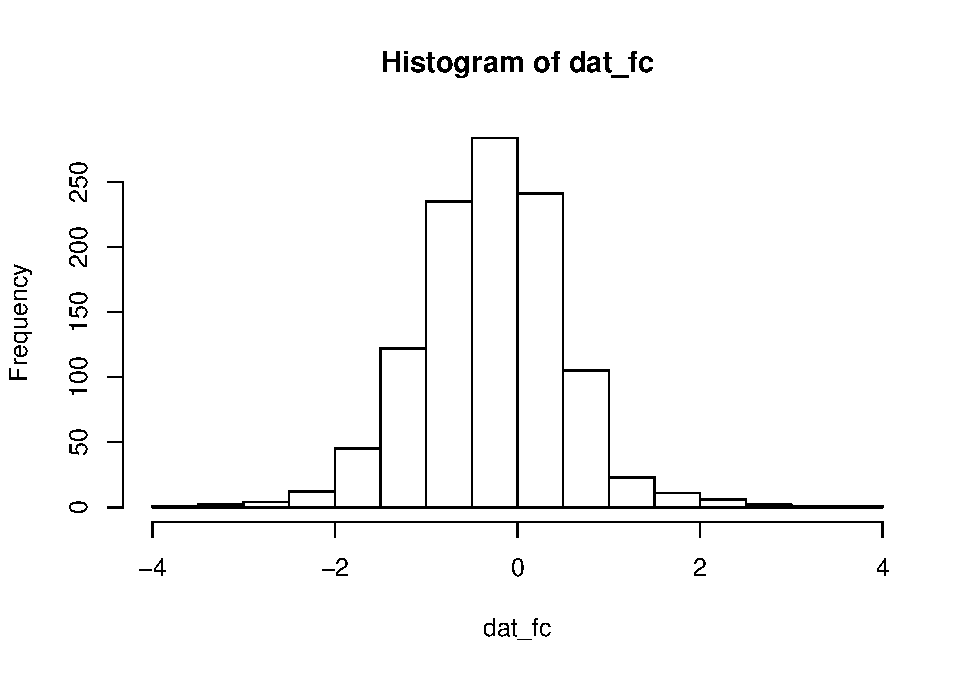
\includegraphics{bspr-workshop-2018_files/figure-latex/fold-change-1.pdf}

\begin{Shaded}
\begin{Highlighting}[]
\KeywordTok{hist}\NormalTok{(dat_max_fc)}
\end{Highlighting}
\end{Shaded}

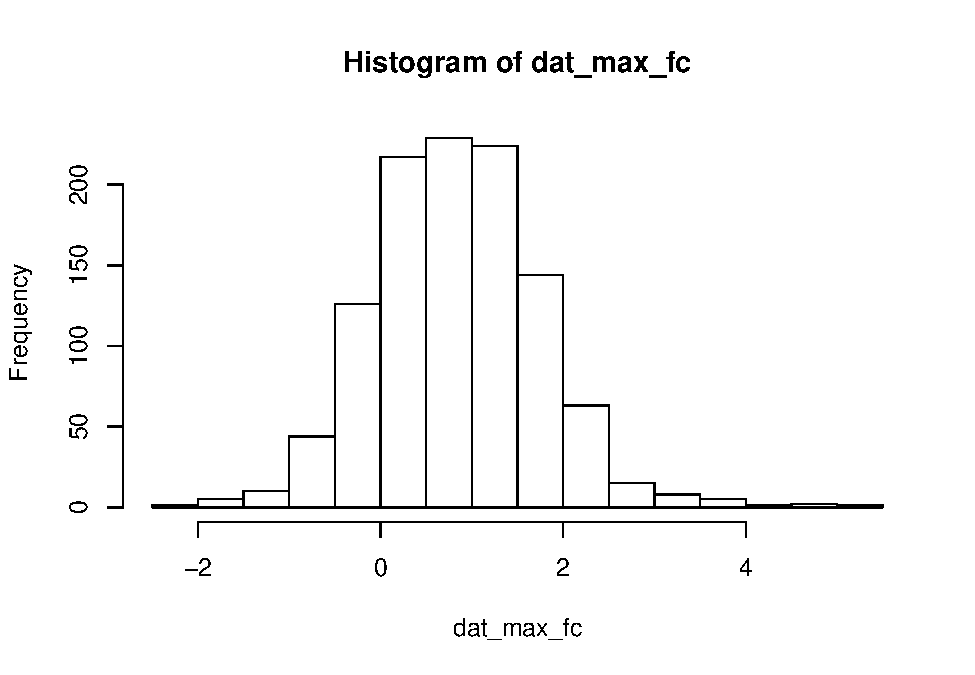
\includegraphics{bspr-workshop-2018_files/figure-latex/fold-change-2.pdf}

\begin{enumerate}
\def\labelenumi{\arabic{enumi}.}
\setcounter{enumi}{6}
\tightlist
\item
  Create a combined table of log fold change and p-values for all the
  proteins for plotting a volcano plot.
\end{enumerate}

\begin{Shaded}
\begin{Highlighting}[]
\NormalTok{dat <-}\StringTok{ }\KeywordTok{data.frame}\NormalTok{(}\DataTypeTok{prots=}\NormalTok{ dat_norm}\OperatorTok{$}\NormalTok{protein_accession,}
                      \DataTypeTok{logfc =}\NormalTok{ dat_fc, }
                      \DataTypeTok{pval =} \OperatorTok{-}\DecValTok{1}\OperatorTok{*}\KeywordTok{log10}\NormalTok{(p_vals))}

\NormalTok{dat_max <-}\StringTok{ }\KeywordTok{data.frame}\NormalTok{(}\DataTypeTok{prots=}\NormalTok{ dat_norm_max}\OperatorTok{$}\NormalTok{protein_accession,}
                      \DataTypeTok{logfc =}\NormalTok{ dat_max_fc, }
                      \DataTypeTok{pval =} \OperatorTok{-}\DecValTok{1}\OperatorTok{*}\KeywordTok{log10}\NormalTok{(p_vals_max))}

\NormalTok{dat_max }\OperatorTok\StringTok{ }\KeywordTok{ggplot}\NormalTok{(}\KeywordTok{aes}\NormalTok{(logfc,pval)) }\OperatorTok{+}\StringTok{ }\KeywordTok{geom_point}\NormalTok{()}
\end{Highlighting}
\end{Shaded}

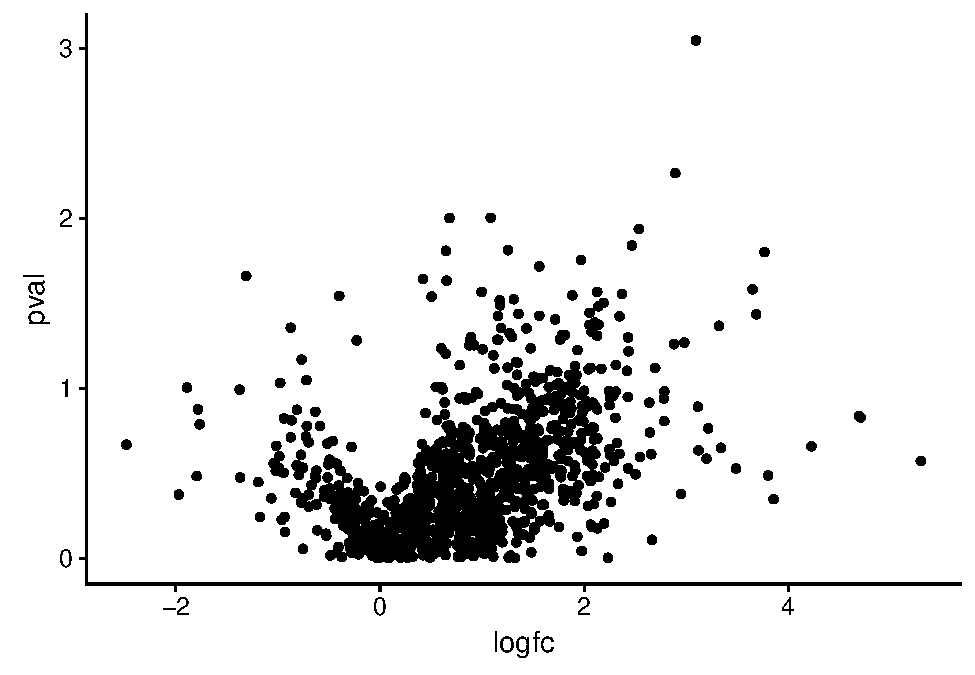
\includegraphics{bspr-workshop-2018_files/figure-latex/vol-pot-1.pdf}

\begin{Shaded}
\begin{Highlighting}[]
\NormalTok{dat }\OperatorTok\StringTok{ }\KeywordTok{ggplot}\NormalTok{(}\KeywordTok{aes}\NormalTok{(logfc,pval)) }\OperatorTok{+}\StringTok{ }\KeywordTok{geom_point}\NormalTok{()}
\end{Highlighting}
\end{Shaded}

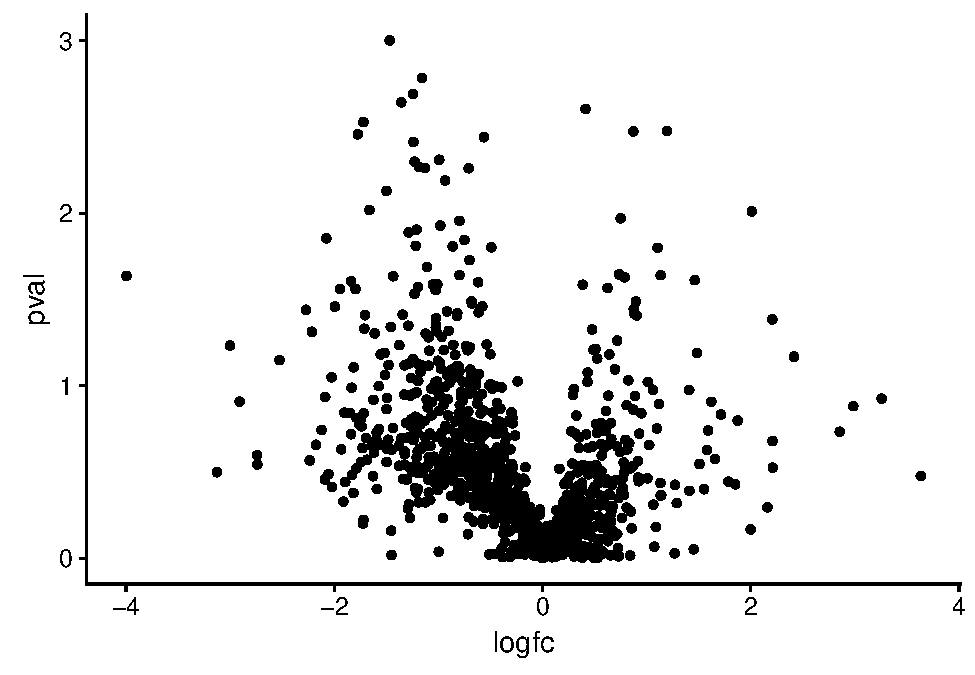
\includegraphics{bspr-workshop-2018_files/figure-latex/vol-pot-2.pdf}

\chapter{Visualising proteomics data}\label{visualising-proteomics-data}

Based on empircal research, there are some general rules on
visulisations that are worth bearing in mind:

\begin{enumerate}
\def\labelenumi{\arabic{enumi}.}
\tightlist
\item
  Plot
\end{enumerate}

\section{Creating a volcano plot}\label{creating-a-volcano-plot}

VOlcano plot is a plot of the log fold change in the observation between
two conditions on the x-axis, for example the protein expression between
treatment and control conditions. And on the y-axis is the corresponding
p-value for each observation. The p-value representing the likelihood
that an observed change is due to the different conditions rather than
arising from natural variation in the fold change that might be observed
if we performed many replications of the experiment.

The aim of a volcano plot is to enable the viewer to quickly see the
effect (if any) of an experiment with two conditions on many species
i.e.~proteins in terms of both increased and decreased expression.

Like all plots it has it's good and bad points, namely it's good that we
can visualise a lot of complex information in one plot. However this is
also it's main weakness, it's rather complicated to understand in one
glance.

However, volcano plots are widely used in the literature, so there may
be an amount of \href{https://en.wikipedia.org/wiki/Social_proof}{social
proof} giving rise to their popularity as opposed to their utility.

\section{Creating a heatmap}\label{creating-a-heatmap}

A

\chapter{Going further}\label{going-further}

\section{Getting help and joining the R
community}\label{getting-help-and-joining-the-r-community}

\section{Communication: creating reports, presentations and
websites}\label{communication-creating-reports-presentations-and-websites}

\bibliography{packages.bib}


\end{document}
